%%%%%%%%%%%%%%%%%%%%%%%%%%%%%%%%%%%%%%%%%%%%%%%%%%%%%%%%%%%%%%%%%%
%%%%%%%% CPSC 68 SPRING 2017 EXAMPLE REPORT %%%%%%%%%%%%%%%%%%%%%%%%
%%%%%%%% This template is modified from ICML 2014 %%%%%%%%%%%%%%%%
%%%%%%%%%%%%%%%%%%%%%%%%%%%%%%%%%%%%%%%%%%%%%%%%%%%%%%%%%%%%%%%%%%

\documentclass{article}

%include any external packages here.  This is similar to loading a
%library in python or C++

% use Times
\usepackage{times}
% For figures
\usepackage{graphicx}
\usepackage{subfigure}

% For citations
\usepackage{natbib}

% For algorithms and pseudocode
\usepackage{algorithm}
\usepackage{algorithmic}

%Adds hyperlinks to your citations automatically
\usepackage{hyperref}

% Packages hyperref and algorithmic misbehave sometimes.  We can fix
% this with the following command.
\newcommand{\theHalgorithm}{\arabic{algorithm}}

\usepackage[accepted]{icml2014}

\usepackage{amsmath}
\usepackage{amssymb}
\usepackage{bm}


% If your title is long (below), use this command to also provide
% short version.  This will go on the top of every page
\icmltitlerunning{Final Report}

\begin{document}

\twocolumn[ %use two column if you need a text to span across the whole page
\icmltitle{Text Classification with Horror Authors}

\icmlauthor{Vickram Rajendran}{vrajend1@swarthmore.edu}
\icmladdress{Swarthmore College, 500 College Avenue, Swarthmore, PA 19081 USA}
\icmlauthor{Caleb Ho}{cho2@swarthmore.edu}
\icmladdress{Swarthmore College, 500 College Avenue, Swarthmore, PA 19081 USA}

\vskip 0.3in
]
\begin{abstract}
Text classification is the supervised learning problem of assigning labels to various snippets
of natural language text. In this paper, we tackle the Kaggle competition
``Spooky Author Identification" in which participants are given sentences from
horror stories written by Edgar Allen Poe, Mary Shelley, and HP Lovecraft, and
tasked with predicting which author wrote a given sentence. We provide a survey
of various text classification algorithms and compare their performance on this
task.
\end{abstract}

\section{Introduction}
\label{introduction}
Text classification belongs to a more general class of problems called sequence
classification. In sequence classification, we are given a set of sequences of letters
over a finite alphabet and a set of labels, and we need to assign a label to each
sequence. This kind of problem appears in many different contexts including
speech recognition and protein sequence classification.

In this paper, we tackle the Kaggle competition ``Spooky Author Identification" in
which we are given a data set of sentences labeled by author in order to train a
model which can correctly identify the author of unseen sentences. Since we are
dealing with natural language text, the features in our data (i.e. the words) are
highly auto-correlated. Hence the algorithms we choose to fit to the data should,
at the very least, not assume feature independence, but also leverage its intrinsic
structure to generate accurate predictions.

This problem was particularly interesting to us because it was a chance for us to
apply our knowledge of supervised learning in a slightly different context.
Many of the algorithms we discussed this semester were not for sequential
data. Thus we wanted to explore various algorithms designed for handling
sequential data, and compare their performance to ones not specialized for this
task.

\section{Related Work}
\label{related-work}

Since many algorithms expect numerical input, an important part of any learning
task with natural language text input is deciding how to embed the input data
into some real space $\mathbb{R}^d$. The task of word embedding can be thought of
as a specific case of dimensionality reduction since the original feature space
is some natural language dictionary with tens of thousands of words which we
want to represent with far fewer dimensions.

One common approach to word embedding is using a bag of words. In bag of words,
we restrict our vocabulary to be the top $d$ words in our corpus and a ``none"
category, resulting in a categorical variable with $d + 1$ levels. Then we
one-hot encode each word in our corpus such that each dimension in
$\mathbb{R}^d$ is a binary variable for a top $d$ word.

Another approach to word embedding is using word2vec which embeds words into 
$\mathbb{R}^d$ such that
the similarity between words can be computed by taking the dot product of word
vectors \cite{word2vec}. In bag of words, word vectors are orthogonal and thus no such notion
of similarity exists. Furthermore, word2vec does not limit the vocabulary size
of the corpus in the way bag of words does.

Another problem related to text classification is topic modelling. In addition to
syntax, natural languages have semantics. Therefore it may be useful to first
reduce input sentences into a list of topics before classifying them. Topics
may offer a more succinct and holistic form of dimensionality reduction which leverages
the inherent structure of natural language.

We utilized two topic modelling algorithms for this project: Latent Dirichlet 
Allocation (LDA) \cite{lda} and non-negative matrix factorization (NMF)
\cite{nnmf}. 
We also tested two other algorithms specifically designed to tackle sequence
classification: a long-short term memory neural network (LSTM)
\cite{lstm}, and a hidden
Markov model (HMM) \cite{hmm}. 

\section{Methods and Methodology}
\label{methods}
\subsection{Exploratory Data Analysis and Preprocessing}
We began the process by performing exploratory data analysis on the data. The goal of this procedure was to determine if there were any clear patterns, both internal and external to the data, that we might need to take into account when testing our algorithms. For instance, it might be possible that Mary Shelley uses some word far more frequently than Edgar Allan Poe - this could imply that some algorithms that take specific word frequency into account like the bag of word embedding scheme might perform better. Or perhaps there were some distributions of the data that could help inform a better prior for the Naive Bayes implementation. Our exploratory data analysis showed that while each author certainly preferred different words, none of the words that they used were significant enough to warrant modifying our instances of the algorithm to account for it. 
\begin{figure}[!ht]
    \centering
    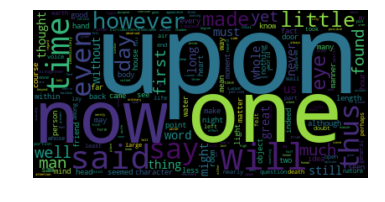
\includegraphics[scale = .5]{eap.png}
    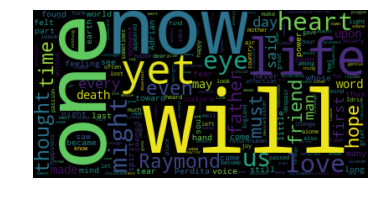
\includegraphics[scale = .5]{mws.png}
    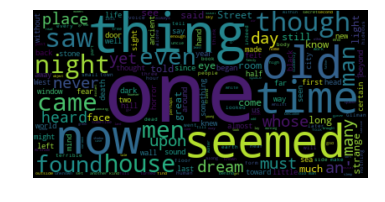
\includegraphics[scale = .5]{hpl.png}
    \caption{Wordclouds made of the training data of (top to bottom) Edgar Allan Poe, Mary Shelley, and HP Lovecraft}
    \label{fig:word_clouds_eda}
\end{figure}

Since we are dealing with natural language text, it was necessary for us to preprocess
our data. This involved removing leading and trailing punctuation, converting everything
into lowercase, and removing stop words (i.e. words which carry little meaning like
``the", ``a", ``this", etc.).

\subsection{Na\"ive Bayes}
\label{nb}
Naive Bayes is a generative model that seeks to predict the distribution of the labels in the feature space. The algorithm begins by using a Maximum A Posterior estimate to determine the probabilities that a label occurs, and the probabilities that a feature occurs given a training label. By making the assumption that the features are independent from each other (The Naive Bayes Assumption), calculating these suffice to calculate the probability that a set of features occurs given a training label. Then by using Bayes Theorem, the algorithm is able to determine the probability that a training label occurs given a set of features. Choosing the training label that has the highest probability will be the prediction of the Naive Bayes Classifier. 

We have constructed two sets of features for the corpus of data that we have but since we perform Naive Bayes on the mean word embedding of the sentence, we have real-valued features. We use a Gaussian Naive Bayes implementation in order to take this into account, which allows for real-valued features and assumes they are in a gaussian distribution. This is the standard implementation of Naive Bayes for real-valued features. In practice, the implementation of Naive Bayes is as follows.


\begin{enumerate}
    \item Calculate the probability that a label occurs in the training data
    \item Calculate the probability that each feature class occurs given a label
    \item Use Laplace smoothing to pre-process the probabilities
    \item Given a new piece of data, calculate the probability that a training label occurs given the feature set (Using Bayes Rule)
    \item Return the label that had the highest probability. 
\end{enumerate}
\subsection{Latent Dirichlet Allocation}
Using LDA for dimensionality reduction has been demonstrated to
not degrade classifer performance, and in most cases improve classifier performance.
\cite{lda}. In a given corpus of documents, LDA assumes that documents are
some mixture of topics, and each word of each document is drawn from some
topic of that document. The generative process for a document 
$\bm{w}$ (a tuple of words) is as follows \cite{lda}.
\begin{enumerate}
    \item Choose a document length $N \sim \text{Poisson}(\xi)$, $\xi \in \mathbb{R}^+$.
    \item Choose a topic mixture $\theta \sim \text{Dir}(\bm{\alpha})$, $\bm{\alpha} \in
    (\mathbb{R}^+)^K$.
    \item For $w_n \in \bm{w} = (w_1, w_2, \ldots, w_N)$:
    \begin{enumerate}
        \item Choose a topic $z_n \sim \text{Multinomial}(1, \theta)$.
        \item Choose $w_n$ with probability $p(w_n \mid z_n; \beta)$ where $\beta$ is
        a $K \times V$ matrix with $\beta_{ij} = p(w_j \mid z_i)$, the probability of
        word $j$ given a topic $i$.
    \end{enumerate}
\end{enumerate}
The training process for LDA involves using an EM procedure to estimate the parameters 
of the distributions described above \cite{lda}. Since LDA is not a classifier on its own, and only fits a model of topics, we will be implementing LDA as follows. First we train the LDA on the training data, creating a model that can take in a sentence and give out the portions of each topic that it is in. Then we will perform Gaussian Na\"ive Bayes on the topics in order to create a model where the input data is jus the topics that we have constructed. In this way we are using LDA as a dimensionality reducer, and then we can use the Naive Bayes classifier to classify the data. Some problems with this include the idea that the Naive Bayes assumption will assume that the topics constructed by LDA are independent from each other, which is not generally the case. However, using Naive Bayes allows us to compare and contrast the power of topic modeling with a standard classifier, as well as give us probabilistic results that we can use to calculate log-odds ratios.  
We will be using sci-kit learn's implementation of LDA in our experimentation. 
\begin{figure}[!ht]
    \centering
    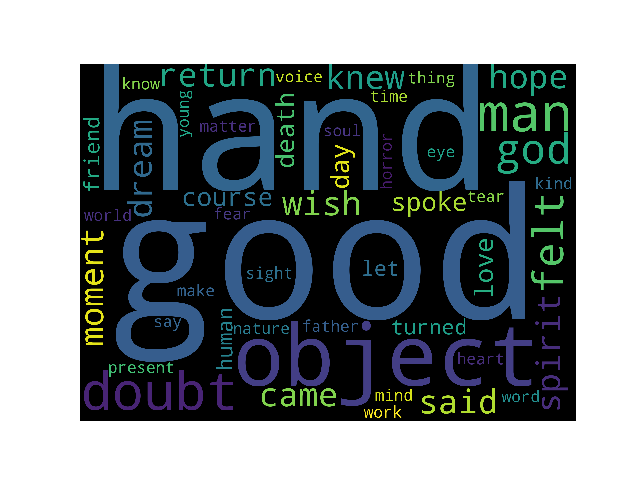
\includegraphics[scale =.5]{lda_topic.png}
    \caption{A topic generated by Latent Dirichlet Allocation}
    \label{fig:lda_topic}
\end{figure}

\subsection{Non-negative Matrix Factorization}

In NMF, we have an $n \times m$ matrix $V$ with non-negative entries which we want 
to approximate as the product of an $n \times r$ matrix $W$ and an $r \times m$ matrix
$H$, both with non-negative entries \cite{nnmf}. The number $r$ is typically chosen so that
$(n + m)r < nm$.  In text classification, the matrix 
$V$ represents
the counts of words in documents; entry $v_{ij}$ of $V$ is the number of occurrences of
word $i$ in document $j$. We can thus regard the columns of $W$ as basis documents (or
topics) and 
the columns of $H$ as an encoding of the documents in $V$ (since each document in $V$
is a linear combination of the basis documents with coefficients specified by a column
in $H$). Similar to LDA, NMF has also shown promise in learning the topics of documents - in particular, NMF has been shown to be able to distinguish the semantics of words. This means that it has distinguished the difference between words in sentences like "I lead a seminar" and "I am holding lead." While the word "lead" is shared between the two, and thus will be encoded the exact same way, it means different things depending on the contex. NMF has been proven to distinguish between the two and put them in different topics \cite{nnmf}.  NMF, as a topic model, suffers from the same problems that LDA does, and so we will also be using NMF as a dimensionality reducer that we will then feed into a Gaussian Naive Bayes classifier. We will be using scikit-learn's implementation of NMF in our experimentation. 
\begin{figure}
    \centering
    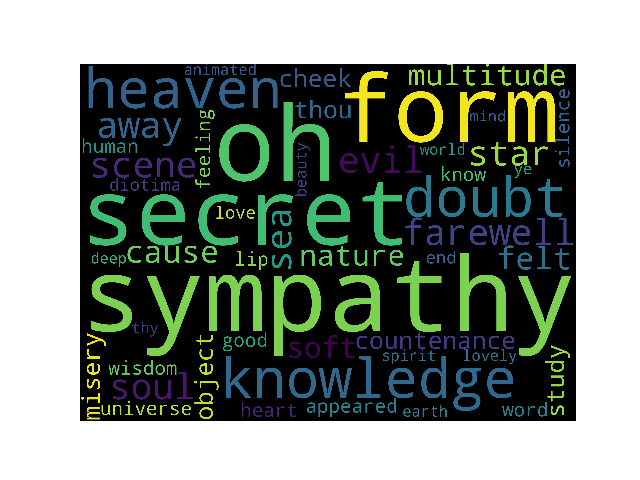
\includegraphics[scale = .5]{nmf_topic.png}
    \caption{An example of a topic generated by Non-negative Matrix Factorization}
    \label{fig:NMF_topic}
\end{figure}

\subsection{LSTM Network}

A neural network is a supervised learning model which can be represented as a
directed acyclic graph comprised of ``layers", see Figure \ref{fig:color_nn}. Each layer
consists of an input vector $\bm{x}$ and a vector of weights $\bm{w}_i$ for each
node $i$ in the subsequent layer. In the simplest case, we have only an input layer
and one output node, so given an input $\bm{x}$ and an output $y$, we want to learn
$\bm{w}$ and $b$ so that $y = \bm{w} \cdot \bm{x} + b$. We can stack layers in this way
where the inputs of hidden layers, i.e. layers in the middle of the network, are the
outputs of the previous layer and the outputs are the inputs to the subsequent layer.
The weights in the network are traditionally learned through gradient descent and 
backpropagation.

\begin{figure}[!ht]
    \centering
    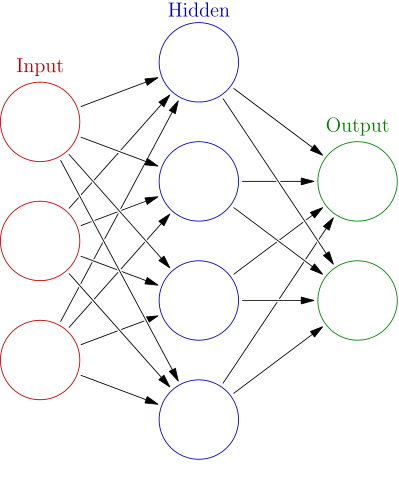
\includegraphics[scale=.45]{Colored_neural_network.png}
    \caption{An example of a neural network with one hidden layer \cite{neuralnetwork}.}
    \label{fig:color_nn}
\end{figure}

Long-short term memory (LSTM) layers are a kind of recurrent layer which squash,
using an activation function, inputs from previous timesteps in addition
to using inputs at the current timestep \cite{lstm}.

Our LSTM network was implemented using Keras \cite{chollet2015keras}. 
Its topology is summarized in Table \ref{tab:lstmtop}. The embedding
layer of our network is responsible for converting sequences of positive
integers into sequences of numerical vectors, e.g. (5, 20, 17) becomes
((.5, .13), (.8, .27), (.34, .44)). Since our network is expecting
sequences of positive integers as input, we mapped each word (after
removing stop words) to an integer.

\begin{table}[!ht]
    \centering
    \begin{tabular}{|c|c|}
        \hline
        Layer & Output Shape \\
        \hline
        Embedding & $20 \times 100$ \\
        LSTM & 20 \\
        Dense & 10 \\
        Dense & 3 \\
        \hline
    \end{tabular}
    \caption{Summary of the topology of our network.}
    \label{tab:lstmtop}
\end{table}

Since the labels for this task are multi-class, the loss function we 
chose was categorical cross entropy. To control for overfitting, we
set the dropout and recurrent dropout of the LSTM layer to be 0.4.

\subsection{Hidden Markov Model}

A (first order) hidden Markov model is a graphical model consisting of hidden and observable
nodes. Each hidden state has transition and emission probabilities. A
transition probability determines the probability of moving to some
other hidden state in the next timestep. An emission probability 
determines the probability of observing some observable node given
the current hidden state. 

\begin{figure}[!ht]
    \centering
    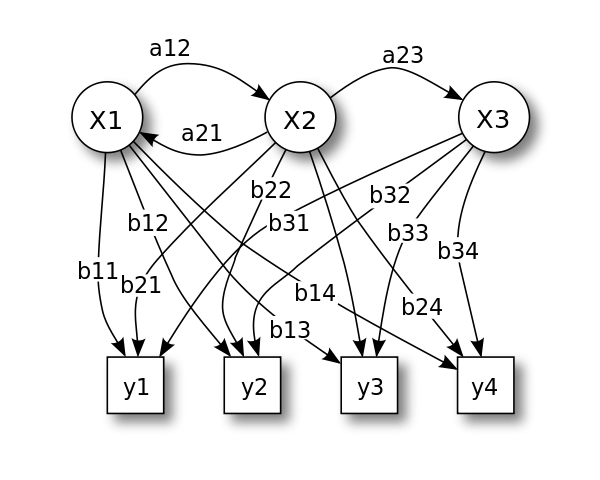
\includegraphics[scale=.4]{HiddenMarkovModel.png}
    \caption{An example of a first order hidden Markov model. The states X1, X2, and X3
    are hidden states; the states y1, y2, y3, and y4 are observed states;
    the weights of edges connecting two hidden states are transition probabilities;
    the weights of edges connecting a hidden state to an output state are
    emission probabilities \cite{hiddenmarkovmodel}.}
    \label{fig:hmm}
\end{figure}

As described, the learning task for an HMM is finding the optimal emission and
transition probabilities given a set of expected output sequences. This can
be formulated into a sequence classification problem \cite{hmm}.



\section{Tuning}
Each of the methods we used have tunable parameters except for Na\"ive Bayes. In order to determine which parameters we should test our model on, the training dataset was split, $90\%$ to the training set, and $10\%$ to a held aside tuning set. Then each algorithm trained with different hyperparameters on the new training set, and tested on the tuning set.  
\subsection{Tuning the Topic Models (LDA, NMF)}
The major hyperparameters in the topic models are the number of iterations, and the number of components. NMF in particular only has the number of components as a tunable parameter, while LDA has both. The number of components are simply the amount of topics that the algorithm will attempt to classify each word into. The number of iterations is the maximum amount of times that the algorithm will try to estimate the variational distribution in the data. Since LDA uses an EM-procedure, if it hasn't converged before the maximum amount of iterations, it will then immediately stop. We expected the accuracy to increase as the number of topics increased, as this would allow the algorithm to create more fine topics, and thus be able to classify the topics more cleanly. We also expected that increasing the maximum number of iterations would not be very useful since LDA has a very fast convergence time \cite{lda}. 
\begin{table}[!ht]
    \begin{center}
\begin{tabular}{|c|c|c|}
    
    \hline
    Number of Topics & Max iters & Tuning Accuracy \\
    \hline
    5 & 3 & 0.486 \\
    5 & 5 & 0.490 \\
    5 & 10 & 0.494 \\
    5 & 15 & 0.495 \\
    10 & 3 & 0.469 \\
    10 & 5 & 0.470 \\
    10 & 10 & 0.472 \\
    10 & 15 & 0.472 \\
    20 & 3 & 0.437 \\
    20 & 5 &0.436 \\
    20 & 10 & 0.437 \\
    20 & 15 & 0.435 \\
    30 & 3 & 0.449 \\
    30 & 5 & 0.448 \\
    30 & 10 & 0.451 \\
    30 & 15 & 0.451 \\
    \hline
    Best: 5 & 15 & 0.495 \\
    \hline
\end{tabular}
\end{center}
    \caption{Tuning LDA - Increasing the number of iterations did comparatively little, fewer topics got higher accuracy}
    \label{tab:tuning_lda}
\end{table}

While we were correct that changing the number of iterations would not affect the data tremendously, our results show that LDA converges to near the maximum in just a few iterations. We were also correct that as the amount of topics increased, the specificity of each topic would increase. For example, when we had 30 topics made by the LDA, words like "heart, love, body, hope, hand, lip, girl, boy, friendships" were all put together, which shows an association that is more than just the general topic of "emotions" or "abstractness". However, when we only had 5 topics, many of those words were split into other, words like "heart, soul, life, death, nature, spirit", and several more subtle associations like that between heart, girl, and boy were missed. Our predictions that increasing the number of topics would help the accuracy were proven very incorrect - while the topics did end up getting more specific, this did not correlate with an increase in performance of LDA. For NMF, however, increasing the topics did increase the performance of the algorithm significantly. Starting at 5 topics yielded an accuracy of only 0.467, but as we increased the number of topics allowed, it reached up to an accuracy of 0.556 at 100 topics before it stagnated and stopped increasing. This was much more aligned with our predictions, and we expect this occurred because NMF was able to more accurately distinguish between topics as the amount of topics increased. We base this conjecture on the fact that LDA allows for more variability with new data since it adds a Dirichlet prior to the data, and since the topics don't seem to have much to do with the actual author (they are all horror authors after all), NMF has a more stable increase with the increase in topics.

\begin{figure}
    \centering
    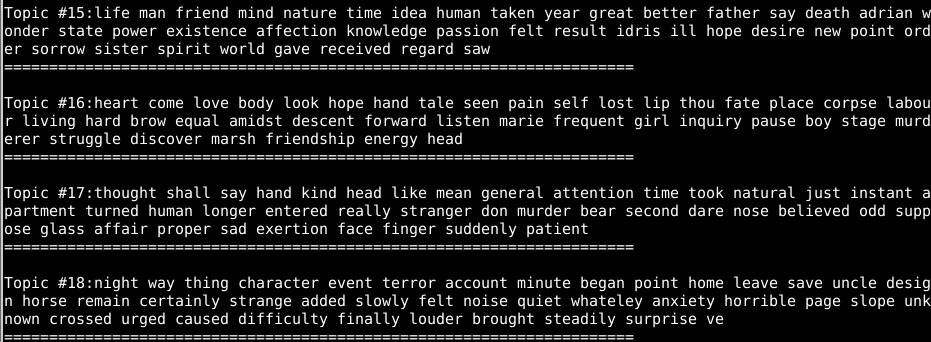
\includegraphics[scale =.25]{topics_30.png}
    \\
    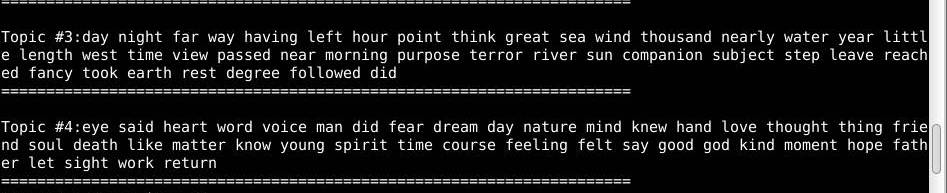
\includegraphics[scale =.25]{topics_5.jpg}
    \caption{Top image is 30 topics, bottom image is 5 topics. The more topics, the more specific the topic content}
    \label{fig:topics_specific}
\end{figure}

\subsection{Tuning the LSTM}

LSTMs are known to quickly overfit, so it was important for us to properly tune
our network. Specifically, we tuned the number of epochs trained and the number
of output units for the LSTM layer as shown in Table \ref{tab:nn-tune}.

\begin{table}[!ht]
    \centering
    \begin{tabular}{|c|c|c|c|}
        \hline
        Epochs & LSTM Units & Tune loss & Tune accuracy\\
        \hline
        5 & 5 & 0.534 & 0.808 \\
        5 & 10 & 0.566 & 0.790 \\
        5 & 20 & 0.499 & 0.804 \\
        10 & 5 & 0.547 & 0.813 \\
        10 & 10 & 0.542 & 0.810 \\
        10 & 20 & 0.555 & 0.814 \\
        20 & 5 & 0.723 & 0.806 \\
        20 & 10 & 0.698 & 0.812 \\
        20 & 20 & 0.748 & 0.808 \\
        \hline
    \end{tabular}
    \caption{Summary of hyperparameter tuning for our neural network. Loss is
    categorical cross-entropy.}
    \label{tab:nn-tune}
\end{table}

We see that in general, tuning loss worsens as the number of epochs increases,
thus confirming the tendency for LSTMs to overfit quickly. Increasing the
number of output units for the LSTM does not drastically affect loss, but
it does decrease loss for networks trained for only five epochs.

\section{Results and Analysis}
\begin{table}[!ht]
    \centering
    \begin{tabular}{|c|c|}
        \hline
        Algorithm & Average Accuracy \\ \hline
        Multinomial Na\"ve Bayes & 0.823  \\
        LDA + Gaussian Naive Bayes & 0.495\\
        NMF + Gaussian Naive Bayes & 0.556  \\
        LSTM & 0.792 \\
        HMM & 0.562 \\ \hline
    \end{tabular}
    \caption{Tuning accuracy of the algorithms}
    \label{tab:results}
\end{table}

\begin{table}[!ht]
    \centering
    \begin{tabular}{|c|c|}
        \hline
        Algorithm &  Categorical Cross-entropy \\
        \hline
        Multinomial Na\"ive Bayes & 0.474 \\
        LDA + Gaussian Naive Bayes& 1.08\\
        NMF + Gaussian Naive Bayes& 6.615 \\
        LSTM & 0.463 \\ 
        HMM & 1.018 \\ \hline
    \end{tabular}
    \caption{Accuracy in terms of Log-Loss}
    \label{tab:results_1}
\end{table}
We expected Na\"ive Bayes to perform the worst of all the algorithms, but that was not true - Naive Bayes ended up being the best of the algorithms that we tried in terms of accuracy, and very competitive in terms of categorical cross-entropy. In particular, we expected Naive Bayes to perform worse than the Topic Models, because the topic models were supposed to perform dimensionality reduction and find the main topics in each of the author's works. One of the reasons that we believe Naive Bayes performed better was the fact that these authors all are speaking about similar topics - they are all horror authors from the same time period, and we saw from the Exploratory Data analysis that there weren't any particular topics that they used, just particular words. This implies that Naive Bayes, which focuses on each word, would perform better than trying to classify the authors in terms of the topics they are writing on, which is what LDA and NMF have done. If the authors were from differing areas, time periods, or even had very distinct writing styles, we suspect that the topic modelling would work well, but in this case it did not. 

Na\"ive Bayes also performed comparably to the sequential models, the LSTM recurrent neural network and the Markov Chain. This was also a surprise to us, as Na\"ive Bayes has no memory or sequential modelling in its algorithm. The only Natural Language processing tool we used for it was vectorizing the word, and yet it was still able to perform at approximately the same level as algorithms that take into account the ordering of the corpus. Our explanation for the success of Na\"ive Bayes comparatively is that they are both learning completely different things that work equally well on the testing data that we obtain. It is not possible for Na\"ive Bayes to be looking at previous words, or even taking into account the order of words since it operates under the Naive Bayes Assumption, and so it must be discovering a pattern in the distribution of words used by each of the authors. The sequential models, on the other hand, are able to determine small sequences of words and predict the likeliness of a word given previous ones (in the case of markov chains), but this implies that their should be specific sequences that some authors do uniquely. We had a medium sized dataset, so most of these distinctive sequences should be accounted for, but since each of the authors were writing about the same topic, it is highly likely that some of the sequences were ambiguous as to which author it could be. However, the sequential models still performed very well, and we expect them to perform even better in situations where the topics are not exactly the same, or if we had a large dataset. 

The sequential models also performed strictly better than the topic models, which only furthers our hypothesis that each of the authors wrote about the same major topics in this corpus. This comes as a little bit of a shock, as even though they all were "horror authors", most authors do have different topics that the topic modelling would pick up on. Some of this can be explained due to the gathering of the data - since the data was for a competition, it stands to reason that the machine that curated the data picked so from similar topics as to make it more difficult for the competitor to find patterns between them. If this were the case, then topic models would certainly perform poorly since there are no distinctive topics among the authors. Even if this were not the case, another reason that sequential models might perform better than the topic models is since authors have distinctive writing styles rather than writing topics - since topics are a more general category, it makes sense that the distinctions between authors might be more easily identifiable based on the structure of their sentences, rather than the content of their words. 

Though the topic models had similar results on accuracy, their categorical cross-entropy were highly different. In particular, the NMF model had incredibly large categorical cross entropy, which means it predicted the wrong answer with very high confidence. LDA, on the other hand, would not be very confident in the wrong answers it predicted. The results seeem to imply that LDA is a better topic model for this problem than NMF, but we must still account for both the very poor accuracy of the topic models, and for the fact that NMF tuned at 100 topics. Since we tuned NMF to maximize accuracy rather than categorical cross-entropy, it makes sense that it performed more poorly than LDA in that area because more topics means that there are more features for the Gaussian Naive Bayes to perform on. Then if some features have high correlation with an author, the model might consider it to be a very important feature even if it has very low frequency - this is much more common with extraneous or redundant features, like having too many topics. In future experiments, we expect that if we train the LDA to find the right number of topics with a measure of categorical-cross entropy rather than just accuracy, the algorithm will find much more success. 

It is also worth noting that of the two sequential models, LSTM performed far better than the hidden markov model. LSTM had an almost 25\% increase in accuracy, and half of the categorical cross-entropy. One reason this might have occurred is due to the HMM only looking one word previously. We did not modify the implementation of HMM that we used to add multiple word memory, so at each step of the markov chain the model was only remembering the previous word. LSTM, on the other hand, propagates it's memory through out the neural network, so while it only looks one "neural net" previously, that neural net has already been updated from the previous one, and so the memory propogates throughout the neural network. This would allow LSTM to have a more complete picture of the sequence, which could account for it performing better. 

\section{Conclusion}
\label{conclusion}

In this paper, we surveyed five different algorithms for text classification.
We found that Multinomial Na\"ive Bayes outperforms methods all methods in
terms of raw accuracy.
Only the LSTM network was able to surpass Na\"ive
Bayes in categorical cross-entropy, but only by a small margin.

Since the sentences in our data set come from authors of the same genre
and similar time periods, we believe topic modeling was not able to effectively
extract discriminating topics between authors. This might explain the effectiveness
of Na\"ive Bayes on our data.

With the exception of Multinomial Na\"ive Bayes, the sequence based
algorithms performed better than the non-sequence based algorithms. This
indicates that certain sequences of words sufficiently discriminate
between authors. Thus a more microscopic approach, i.e. looking at 
sequences of words, has some merits of over more macroscopic approaches
such as looking the topics of a sentence.

Finally, we found that categorical cross-entropy offers a different perspective
into classifier performance from raw accuracy. Unlike accuracy, categorical
cross-entropy heavily penalizes confidently incorrect predictions and thus
offes a more nuanced summary of performance. In the case of Multinomial
Na\"ive Bayes versus the LSTM network, we see that Na\"ive Bayes attains a
higher accuracy, but a higher categorical cross-entropy than the LSTM network.
Hence Na\"ive Bayes was in general more confident about its predictions than
the LSTM, but not necessarily in the right direction.

\section*{Acknowledgments}


We give thanks to Professor Ameet Soni, who's help in both ensuring we remained on task as well as providing valuable insight into topic modelling made this paper possible. 

We would also like to thank Kaggle for curating the dataset, providing a active source of discussion about Natural Language Processing, and creating the competition that this paper has aimed to solve. 



% In the unusual situation where you want a paper to appear in the
% references without citing it in the main text, use \nocite
% \nocite{langley00}

\bibliography{references}
\bibliographystyle{icml2014}

\end{document}


% This document was modified from the file originally made available by
% Pat Langley and Andrea Danyluk for ICML-2K. This version was
% created by Lise Getoor and Tobias Scheffer, it was slightly modified
% from the 2010 version by Thorsten Joachims & Johannes Fuernkranz,
% slightly modified from the 2009 version by Kiri Wagstaff and
% Sam Roweis's 2008 version, which is slightly modified from
% Prasad Tadepalli's 2007 version which is a lightly
% changed version of the previous year's version by Andrew Moore,
% which was in turn edited from those of Kristian Kersting and
% Codrina Lauth. Alex Smola contributed to the algorithmic style files.
